\documentclass[12pt]{article}
\usepackage[utf8]{inputenc}
\usepackage[T2A]{fontenc}
\usepackage[russian]{babel}
\usepackage{amsmath}
\usepackage{amssymb}
\usepackage{dsfont}
\usepackage[dvipsnames]{xcolor}
\usepackage{setspace}
\usepackage{multirow}
\usepackage[a4paper, outer=1.5cm, inner=1.5cm, top=1cm, bottom=1cm]{geometry}
\usepackage{graphicx}
\usepackage{skull}
\usepackage{wasysym}
\usepackage{float}
\graphicspath{{.images/}}
\usepackage{hyperref}
\hypersetup{colorlinks=true, linkcolor=blue, filecolor=magenta, urlcolor=cyan}
\usepackage[firstpage]{draftwatermark}
\SetWatermarkText{
    $\qquad\qquad\qquad\qquad\qquad$\parbox{7cm}{\begin{center}
    
\includegraphics[width = 0.08\textwidth]{lion-logo.png}\bigskip\\~\bigskip\\~\vspace{-24mm}\\~\end{center}}
}
\SetWatermarkAngle{0}
\SetWatermarkScale{1.5}
\usepackage{etoolbox}

\newtoggle{ifsolved}
\newtoggle{needhelp}
\newcounter{num}
\setcounter{num}{1}

\newcommand{\newnum}{\par\textbf{\textnumero\arabic{num}}\stepcounter{num}}
\newcommand{\sol}{\vspace{3mm}\par\textbf{Решение: }}
\newcommand{\ans}{\vspace{3mm}\par\textbf{Ответ: }}
\newcommand{\hint}{\vspace{3mm}\par\textbf{Подсказка: }}
\newcommand{\mode}[1]{
\ifstrequal{#1}{0}{\togglefalse{ifsolved}\togglefalse{needhelp}}{\ifstrequal{#1}{1}{\togglefalse{ifsolved}\toggletrue{needhelp}}{\ifstrequal{#1}{2}{\toggletrue{ifsolved}\togglefalse{needhelp}}{\toggletrue{ifsolved}\toggletrue{needhelp}}}}} %if 0 - if 1 - if 2 - else
%\newenvironment{problem}[8]{%#1, #2, #3
%\parbox{\linewidth}{\vspace{4mm}\ifstrequal{#4}{(лёгкая)}{\newnum\textbf{.}}{\newnum\textbf{*.} } \\ #5}
%\iftoggle{ifsolved}{\sol #6}{}
%\iftoggle{ifsolved}{\ans #7}{}
%\iftoggle{needhelp}{\hint #8}{}}

\newenvironment{problem}[8]{%#1, #2, #3
\parbox{\linewidth}{\vspace{5mm}\ifstrequal{#4}{(лёгкая)}{\newnum\textbf{.}}{\newnum\textbf{*.} } \\ #5}
\iftoggle{ifsolved}{\sol #6}{}

\iftoggle{ifsolved}{\parbox{\linewidth}{\ans #7}}{}
\iftoggle{needhelp}{\parbox{\linewidth}{\hint #8}}{}}

\newenvironment{mylist} %custom list
{ \begin{itemize}
    \setlength{\itemsep}{0pt}
    \setlength{\parskip}{0pt}
    \setlength{\parsep}{0pt}     }
{ \end{itemize}                  }

\newenvironment{homeass}[1]{\vspace*{-1.5cm}
\iftoggle{ifsolved}{
    \section*{\center{Решение домашнего задания к #1.}}
}{
    \section*{\center{\textcolor{Sepia}{Домашнее задание к #1}}}
} \vspace{7mm}\large}

\parindent=0pt
\pagestyle{empty}
%$\!$[\arabic{class}.\arabic{num}]
%\ifnumcomp{\value{counter}}{>}{1}{true}{false}
%\definecolor{Gray}{gray}{0.9}
%\definecolor{mypink}{RGB}{219, 48, 122}
%\newcolumntype{g}{>{\columncolor{Gray}}p{2.8cm}}

\begin{document}
\large
\mode{7}
%0 for problems without hints
%1 for problems + hints
%2 for problems + solutions + answers
%else: show all

{\centering\section*{СПИСОК ЗАДАЧ}}

{\centering\subsection*{\smallskip\\\textcolor{green}{\textbf{Полезные вещи, которые можно и нужно копипастить:}}}}

\subsection*{\textcolor{Emerald}{\textbf{Полезные шпаргалки по LaTeXу:}}}

\textbf{Пример вставки рисунка:}

\begin{minipage}{\linewidth}
    \begin{minipage}{0.54\linewidth}
    см. рисунок справа\\
    Текст к собственно пикче, примерно всегда это либо развёрнутое описание, либо большая часть решения задачи --- стремимся экономить пространство, если это можно сделать.
    \end{minipage}
    \hspace{0.05\linewidth}
    \begin{minipage}{0.4\linewidth}
    \begin{figure}[H] 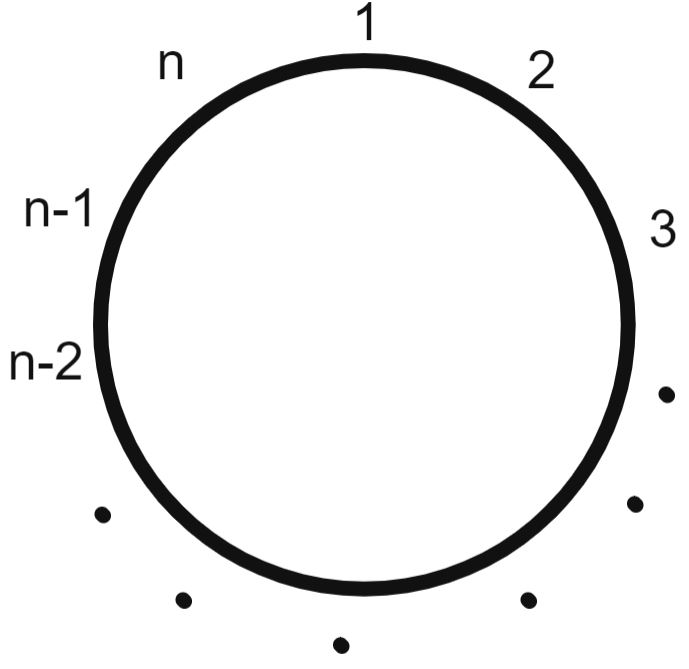
\includegraphics[width=\linewidth]{sol3} %тут поменять имя пикчи
    \end{figure}
    \end{minipage}
\end{minipage}

\textbf{Дефолтные математические знаки и символы:}\\
$\geqslant$,
$\leqslant$,
$a^{b}$,
$x_{i}$,
$\sqrt{a}$,
$\frac{a}{b}$,
$\displaystyle \frac{a}{b}$,
$\cdot$
$\;\Rightarrow\;$,
$\;\Leftrightarrow\;$,
$1{,}2$.
О промежутках:
$a\!b$,
$a\,b$,
$a\:b$,
$a\;b$,
$a\quad b$.

\textbf{Стандартные система и совокупность уравнений / неравенств:}\\
$\left\{
\begin{aligned}
f(x) &= 0 \\
g(x) &= 1
\end{aligned}\right.$

$\left[\begin{aligned}
&\left\{\begin{aligned}
f(x) &\geqslant a \\
g(x) &= b
\end{aligned}\right.\\
&\left\{\begin{aligned}
f(x) &< a \\
g(x) &= -b
\end{aligned}\right.
\end{aligned}\right.$

\subsection*{\textcolor{Emerald}{\textbf{Не математическое, но полезное:}}}
% комментарий в любом месте документа, который нигде не будет видно. Можно использовать для написания заметок-вопросов по задачам
\textbf{Пример таблицы:}

\begin{tabular}{|c|c|c|}
\hline
    $a$ & $b$ & текст
\\\hline
    $c$ & $d$ & мораль
\\\hline
\end{tabular}\\

\textbf{Отступы:} между\smallskip\\ строками\medskip\\ \textbf{Тире} --- это три дефиса.\\
\textbf{Списки:}
\begin{mylist}
\item [$\bullet$] это был пункт а
\item [2)] а это уже пункт номер 2 с изменённым заголовком
\end{mylist}

\subsection*{\textcolor{Emerald}{\textbf{Всё, неупомянутое выше (или если просто что-то не так):}}}
\begin{mylist}
\item [$\bullet$] Решение отдельных вопросов касательно ТеХа нужно искать в \href{https://www.mccme.ru/free-books/llang/newllang.pdf}{Львовском}.

\item [$\bullet$] Найти произвольный символ, который нужен, можно в \href{http://detexify.kirelabs.org/classify.html}{Detexify}.

\item [$\bullet$] Если возникли сомнения при решении, ответ практически ко всем задачам можно проверить с помощью \href{https://www.wolframalpha.com/}{WolframAlpha}.

\item [$\bullet$] Если в задаче нужно создать картинку, то лучше пока отложить эту задачу. Все графики планируется централизованно нарисовать (или перерисовать) в геогебре.

\item [\textcolor{brown}{\textbf{!!}}] Важно ставить \textcolor{red}{\textbf{$\spadesuit$}}
(или просто red) в тело задачи в случае серьёзных вопросов к решению и какой-то вопиющей лажи.

\item [\textcolor{brown}{\textbf{!!}}] Важно ставить \textcolor{olive}{\textbf{$\spadesuit$}}
(или просто olive) в тело задачи в случае не самого удачного текста и кривых отступов.
\end{mylist}

\subsection*{\textcolor{Violet}{\textbf{Комментарии:}}}% а также невидимые комментарии - так можно оставлять заметки-вопросы прямо в задаче, чтобы потом было понятно, в чём вопрос.
\begin{mylist}
\item [$\skull$] Переставлять задачи местами --- очень плохая идея.

\item [$\smiley$] При двойном клике по тексту pdf справа происходит автоматический переход к этому месту в латех-коде, а для обратного перехода можно нажать стрелку вправо (висит сверху между pdf и латех-кодом).

\item [$\smiley$] Если есть размышления, дописывать red/olive к задаче или не дописывать, то лучше всё-таки дописать.

\item [$\skull$] Самое плохое, что можно сделать --- написать в любое поле из трёх (НаписанноеРешение/ВерныйОтвет/Подсказка) только половину того, что надо, никак это не отметить, и потом пойти дальше.\\ Нужно в этот момент писать red/olive в случайном месте задачи, чтобы потом вычислить это с помощью Ctrl+F по всему документу (и это то, что потом будет делаться долго и тщательно)
\end{mylist}

\newpage
\setcounter{num}{434}

\hypertarget{6.9}{{\centering\section*{\bigskip\\\textcolor{Blue}{\hyperlink{start2}{\textcolor{Blue}{6.9}} Координаты и графики.}\vspace{-5mm}}}}

\begin{problem}{Перпендикулярные прямые (напоминание про прямые и развернутые углы).}{6.9.1}{6K}{(лёгкая)}
{\vspace{-13mm}\\\begin{minipage}{\linewidth}
    \begin{minipage}{0.58\linewidth}
    \vspace*{6mm}
    Справа изображены три четырёхугольника.\smallskip\\ Перерисовать каждый из них в тетрадь, и для каждого провести через точку $B$ и через точку $M$ прямые, перпендикулярные прямой $AD$, а через точку $K$~--- прямую, перпендикулярную прямой $CD$.
    \end{minipage}
    \hspace{0.04\linewidth}
    \begin{minipage}{0.36\linewidth}
        \begin{figure}[H]
        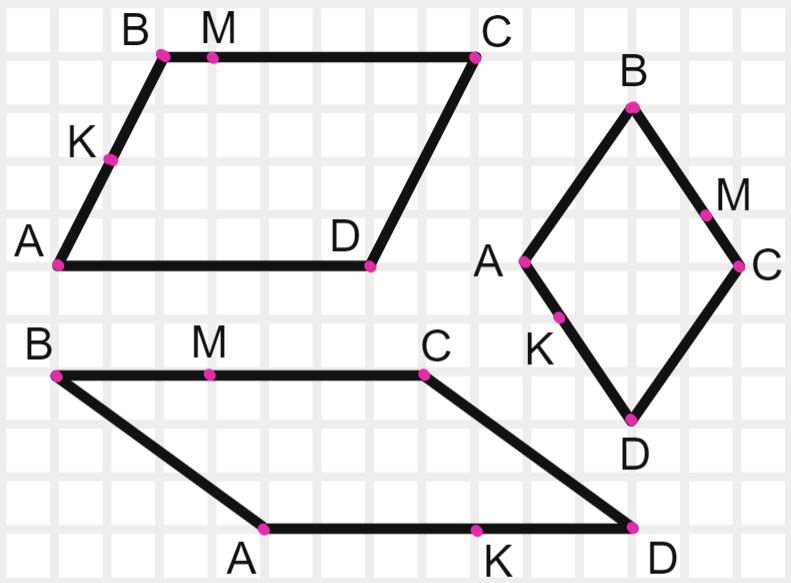
\includegraphics[width=\linewidth]{6K-5}
        \end{figure}
    \end{minipage}
\end{minipage}}
{НаписанноеРешение}
{ВерныйОтвет}{Подсказка}
\end{problem}

\begin{problem}{Координатная плоскость.}{6.9.3}{6K}{(лёгкая)}
{Нарисовать на координатной плоскости точки с координатами $(-4; -2)$, $(-4; 2)$, $(-2; -1)$, $(0; 2{,}5)$, $(2; -1)$, $(4; 2)$, $(4; -2)$. Соединить. Что получилось?}
{НаписанноеРешение}
{ВерныйОтвет}{Подсказка}
\end{problem}

\begin{problem}{Координатная плоскость.}{6.9.3}{6K}{(лёгкая)}
{a) Нарисовать на координатной плоскости прямую, параллельную оси $x$, но находящуюся выше неё на 3 клетки.\\
b) Нарисовать на координатной плоскости прямую, параллельную оси $y$, но находящуюся левее неё на 2 клетки.\\
с) Нарисовать на координатной плоскости прямую, перпендикулярную оси $y$, но находящуюся ниже оси $x$ на 1 клетку.\\
d) Нарисовать на координатной плоскости прямую, перпендикулярную оси $x$, которая проходит через точку $(2; 4)$.}
{\vspace{-5mm}\\\begin{minipage}{\linewidth}
    \begin{minipage}{0.54\linewidth}
    \vspace{7mm}
    Нарисуем прямые (а) и (b), сдвинув их на три клетки вверх и на две клетки влево,\\ соответственно (см. рисунок справа).\\
    Прямая в пункте (с) перпендикулярна оси $y$, а значит идёт параллельно оси $x$, на одну клетку ниже оси.\\
    В пункте (d) прямая перпендикулярна оси $x$, поэтому она будет параллельна оси $y$.\\ Она проходит через точку $(2; 4)$, а значит прямая сдвинута на две клетки вправо.
    \end{minipage}
    \hspace{0.02\linewidth}
    \begin{minipage}{0.43\linewidth}\begin{figure}[H] 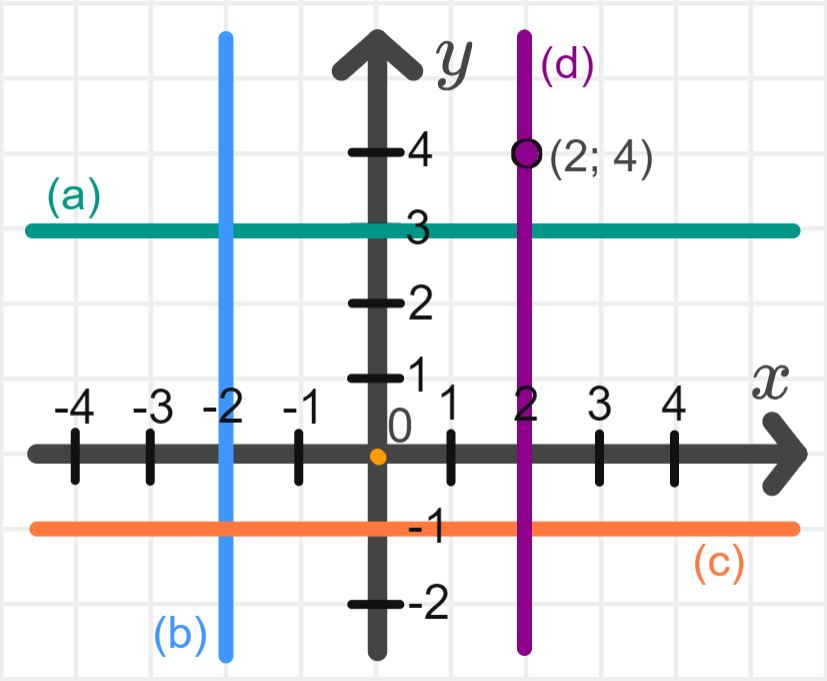
\includegraphics[width=\linewidth]{sol8}\end{figure}\end{minipage}
\end{minipage}}
{Прямые изображены на рисунке выше.}{Если прямая перпендикулярна одной координатной оси, то что можно сказать про эту прямую и другую координатную ось?}
\end{problem}

\begin{problem}{Координатная плоскость.}{6.9.3}{6K}{*}
{Нарисовать на координатной плоскости все точки $(x; y)$, у которых: 
\\a) $x = 2$, а $y$~--- любое; \hfill b) $y = -3$, а $x$~--- любое; \hspace*{2.3cm}\\ c) $x \geqslant 1$, а $y$~--- любое;
\hfill d) $y \geqslant 2$, а $x$~--- любое;\hspace*{2.3cm}$\,\quad$ \\ e) $x \geqslant 1$ и $y \geqslant 2$ одновременно; \hfill f) $x = 2$, а $y \geqslant -1$ одновременно?}
{НаписанноеРешение}
{ВерныйОтвет}{Подсказка}
\end{problem}

\begin{problem}{Координатная плоскость.}{6.9.3}{6K}{(лёгкая)}
{Нарисовать на координатной плоскости точки $A$ и $B$ с координатами $A = (0; 2)$ и $B = (1; 1)$. Придумать любое число, а затем вычислить второе число, такое, что сумма этих двух чисел равна $2$. Где находится точка с этими координатами? Отметить её на плоскости, повторить ещё несколько раз.\\ Какова закономерность? Что получилось? Почему?}
{НаписанноеРешение}
{ВерныйОтвет}{Подсказка}
\end{problem}

\begin{problem}{Координатная плоскость.}{6.9.3}{6K}{(лёгкая)}
{Творческая задача: придумать как можно больше ситуаций, где несколько чисел/букв (координат) определяют место/текущую ситуацию/состояние. \\ Пока что, рекорд по этой задаче~--- 6 примеров :) $\quad$ К примеру: улица, номер дома и номер квартиры (но не подъезда!) точно определяют адрес в Москве.

}
{Примеры ситуаций:\\
0) Полный адрес для отправки письма или открытки из любой страны:\\ страна-город-улица-дом-квартира (Но не корпус или этаж!!)\\
1) В кинотеатре: номер зала определяет зал, номер ряда определяет ряд, номер места определяет, куда мы в итоге сядем. Итого, всего 3 числа: (зал; ряд; место).\\
2) Координатная плоскость, когда пара чисел $(x; y)$ определяет и смещение вправо-влево, и смещение вверх-вниз.\\
3) Координаты на шахматной доске, a1-h8: буква отвечает за одно направление, цифра за другое.\\
4) Координаты при игре в морской бой.\\
5) Координаты на глобусе (в градусах северной/южной широты и восточной/ западной долготы); к примеру, координаты парка Зарядье: (N$\,$55,751$^\circ$; E$\,$37,629$^\circ$).\\
6) (сложный)~--- на любом электронном устройстве любой видимый цвет получается смешением красного, зеленого, и синего (модель RGB). В результате каждый цвет записывается как $(r; g; b)$, числа задают количество каждого цвета.
}
{В большинстве случаев примеры так или иначе связаны с плоской картинкой и движением вверх-вниз и вправо-влево.}{Набор координат может состоять и из одного числа, и из нескольких~--- главное, чтобы ситуация была зафиксирована.}
\end{problem}

\begin{problem}{Координатная плоскость.}{6.9.3}{6K}{*}
{a) Отметить точку $A$ с координатами $(5; 2)$~--- это деревня Болотово;
\\b) Нарисовать синим точки на прямой, которые являются решениями уравнения $y = 3x - 3$~--- это река, которая проходит рядом с деревней;
\\c) Отметить зелёным область, где $4 \leqslant x \leqslant 9$ и $3 \leqslant y \leqslant 7$ (одновременно)~--- это поле, где выращивают капусту.
\\Известно, что напротив деревни, ровно на таком же расстоянии от реки как и деревня, но с другой стороны реки, стоит радиовышка. Нарисовать, где она находится, найти её координаты. Какое расстояние от деревни до поля?\\ А от поля до реки? Как мы тогда выяснили, где находится радиовышка?}
{\vspace{-5mm}\\\begin{minipage}{\linewidth}
    \begin{minipage}{0.54\linewidth}
    \vspace{7mm}
    Отмечаем деревню Болотово.\\
    Прямая $y = 3x - 3$ (река) проходит через точки $(0; -3)$ и $(1; 0)$~--- дальше можем просто соединить точки и получить прямую (см. рисунок справа)\\
    Поле изображено на рисунке справа;\\ координаты радиовышки~--- $(-1; 4)$.\\
    Мы не можем вычислить расстояние ни от деревни до реки, ни от поля до реки.\\ Но так как радиовышка находится на точно таком же расстоянии, мы просто рисуем точно такой же отрезок (симметрия относительно реки). От деревни до поля~--- 1 км.
    \end{minipage}
    \hspace{0.02\linewidth}
    \begin{minipage}{0.43\linewidth}\begin{figure}[H] 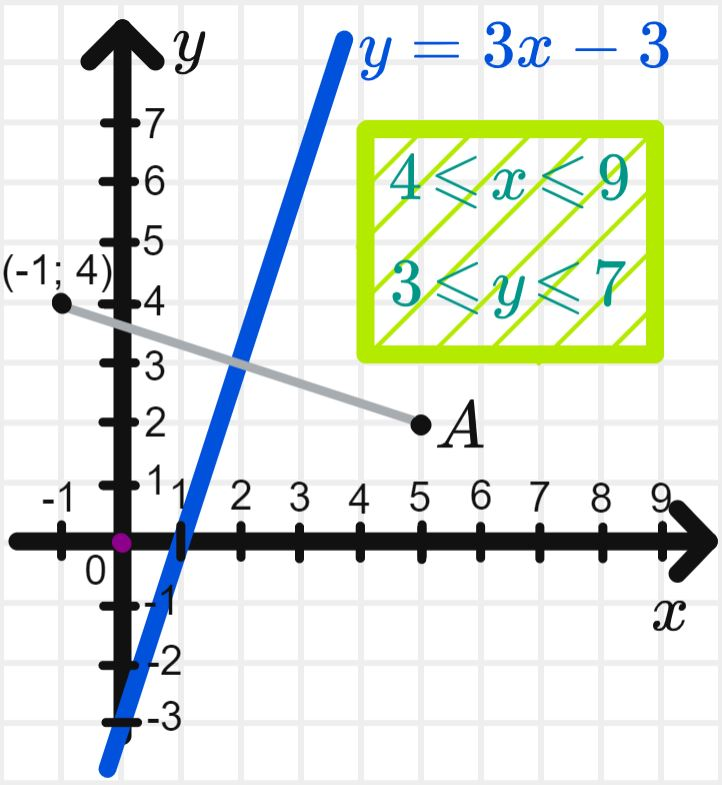
\includegraphics[width=\linewidth]{sol9}\end{figure}\end{minipage}
\end{minipage}}
{Смотри график выше.}{Радиовышка симметрична деревне относительно реки.}
\end{problem}

\begin{problem}{Координатная плоскость.}{6.9.3}{6K}{*}
{Известны координаты нескольких вершин прямоугольника: $(-1; 1)$, $(1; 0)$, $(1; 5)$. Нарисовать прямоугольник, найти координаты его четвёртой вершины и его площадь, если все координаты посчитаны в метрах.\\ Где будет находиться фигура, симметричная ему относительно прямой $x = 4$?\\ А относительно прямой $y = 1$?}
{\vspace{-8mm}\\\begin{minipage}{\linewidth}
    \begin{minipage}{0.51\linewidth}
    ~\vspace{7mm}\\
    Рисунок изображён справа. Можно догадаться, что угол $BAD$~--- прямой, и найти вершину $C$: её координаты равны $(3; 4)$.\smallskip\\
    Для того, чтобы найти его площадь, можно схитрить: разрежем его на 4 треугольника, из которых можно собрать прямоугольник $2\times5$ (линии разреза изображены серым). Получается, что площадь этого прямоугольника равна 10.\\
    Симметричные фигуры получаются отражением по горизонтали и вертикали: это зелёный и оранжевый прямоугольники.
    \end{minipage}
    \hspace{0.04\linewidth}
    \begin{minipage}{0.44\linewidth}
        \begin{figure}[H]
        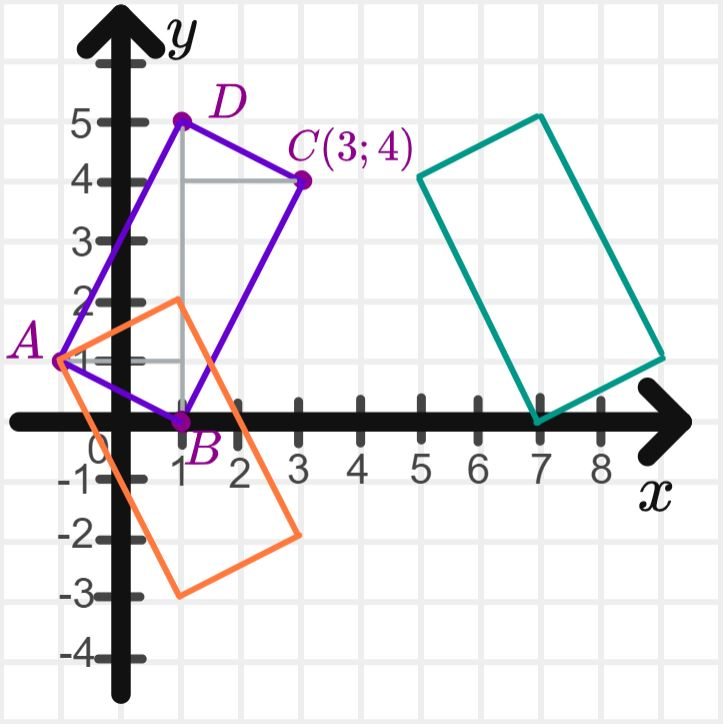
\includegraphics[width=\linewidth]{sol17}
        \end{figure}
    \end{minipage}
\end{minipage}}
{Четвёртая вершина имеет координаты $(3; 4)$, площадь всего прямоугольника равна 10. $\quad$ \textbf{Важно:} Стороны этого прямоугольника НЕ РАВНЫ 2 и 5.}{Для нахождения площади полезно разрезать этот прямоугольник на четыре треугольника.}
\end{problem}

\begin{problem}{Координатная плоскость.}{6.9.3}{79I}{*}
{Найти площадь фигуры $ABCD$, если известны координаты всех точек:\\ $A (-3; -1)$, $\,B (-1; -4)$, $\,C (5; 0)$, $\,D (3; 3)$.}
{НаписанноеРешение}
{ВерныйОтвет}{Подсказка}
\end{problem}

\begin{problem}{Координатная плоскость.}{6.9.3}{9I}{*}
{На координатной плоскости находятся четыре точки: $\mathbb{Z}$, $\mathbb{E}$, $\mathbb{R}$, $\mathbb{O}$. Точка $\mathbb{O}$~--- начало координат, точка $\mathbb{R}$ имеет координаты $(1; 0)$, $\mathbb{E}$~--- координаты $(0; -1)$.\\ В начальный момент времени точка $\mathbb{Z}$ имеет координаты $(-1; 6)$. После этого точка $\mathbb{Z}$ начинает плавно сползать вниз со скоростью 1кл/мин (то есть во всё время движения $x_Z = -1$, а $y_Z$ каждую минуту уменьшается на 1.).\\ Так она скользит ровно 10 минут, после чего останавливается.\\
a) Какова площадь треугольника, образованного точками $\mathbb{Z}$, $\mathbb{E}$, $\mathbb{R}$ в начальный момент времени?
\\b) Какова площадь треугольника $\mathbb{Z}\mathbb{E}\mathbb{R}$ в конечный момент времени?
\\c) Какую часть времени из этих 10 минут точка $\mathbb{O}$ находится внутри треугольника $\mathbb{Z}\mathbb{E}\mathbb{R}$?
\\d) Чему равно наименьшее значение площади треугольника $\mathbb{Z}\mathbb{E}\mathbb{R}$ за эти 10 минут?
\\e) Сколько раз за эти 10 минут площадь треугольника $\mathbb{Z}\mathbb{E}\mathbb{R}$ будет целым числом? (начальный и конечный моменты времени тоже учитываются)}
{НаписанноеРешение}
{ВерныйОтвет}{Подсказка}
\end{problem}

\begin{problem}{Координатная плоскость.}{6.9.3}{6K}{*}
{На рынке в Багдаде происходит что-то странное: один неизвестный старик меняет старые лампы на новые: либо забирает две старые лампы и отдаёт одну новую, либо забирает одну старую лампу и отдаёт взамен две новых.\\ Другой старик, наоборот, меняет новые лампы на старые: либо забирает две новых лампы, а взамен отдаёт одну старую лампу и одну монету, либо забирает одну новую лампу и взамен отдаёт две старых.
\\На рынок пришёл Алладин с одной старой лампой. Сможет ли он:
\\a) Уйти с рынка с $10$ новыми лампами, избавившись от ВСЕХ старых ламп?
\\b) Заработать столько монет, чтобы построить себе роскошный дворец?
\\c) Избавиться от совершенно всех ламп?
\\d) Сделать так, чтобы старых и новых ламп было поровну?}
{\vspace{-8mm}\\\begin{minipage}{\linewidth}
    \begin{minipage}{0.51\linewidth}
    ~\vspace{7mm}\\
    Довольно логично обозначать текущее состояние Алладина, когда у него $m$ старых ламп и $n$ новых ламп, парой чисел $(m; n)$~--- поэтому нарисуем координатную плоскость (смотри рисунок справа).\\ Стартует Алладин из точки $(1; 0)$, с одной старой лампой.\smallskip\\
    a) Для того, чтобы выполнить это условие, нужно попасть в точку $(0; 10)$ (на рисунке обозначена красным).\\ Однако все возможные обмены (4 штуки) образуют <<сетку>>, указанную на рисунке.\\ Очевидно, что точка $(0; 10)$ не находится на этой сетке. Следовательно, попасть в неё Алладин не сможет.\smallskip
    \end{minipage}
    \hspace{0.02\linewidth}
    \begin{minipage}{0.47\linewidth}
        \begin{figure}[H]
        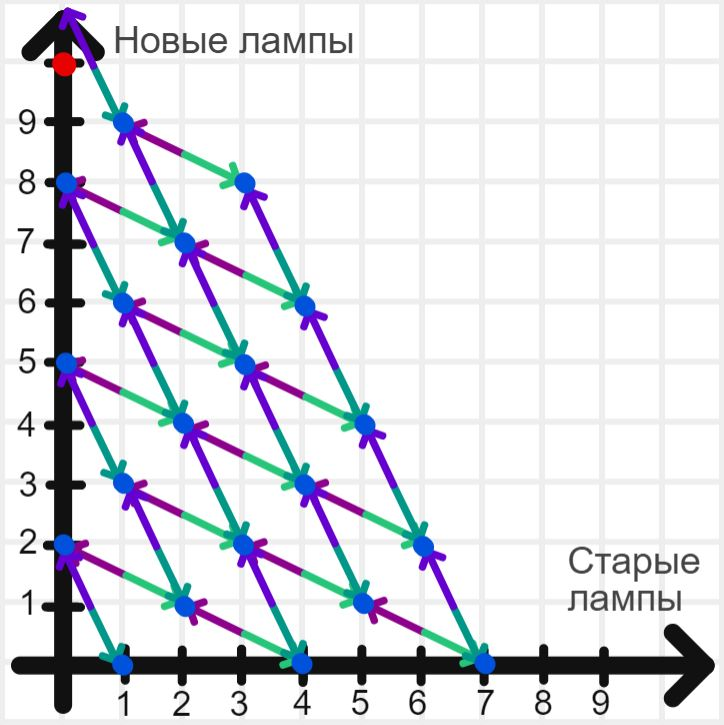
\includegraphics[width=\linewidth]{sol20}
        \end{figure}
    \end{minipage}
\end{minipage}
b) Алладин может вначале менять две новые лампы на старую лампу и одну монету, а потом менять обратно одну старую лампу на новую. В итоге богатство Алладина будет неограниченно расти, и он сможет купить себе любой дворец.\smallskip\\
c) При каждом обмене Алладин получает какую-то лампу (может быть старую, может быть новую). Следовательно, в конце каждого обмена у него есть какая-то лампа, и совсем без ламп он остаться не может.\smallskip\\
d) Если количество старых и новых ламп будет одинаково, то на графике $y = x$ (можно нарисовать прямую). Как мы видим, ни одной точки сетки на этой прямой нет, поэтому логично ожидать, что это невозможно. Докажем это.\\
Рассмотрим разницу между числом старых и числом новых ламп. В ходе обмена двух старых ламп на одну новую или одной старой лампы на две новых эта разница уменьшается на 3. В ходе же обмена одной новой лампы на две старых или двух новых ламп на одну старую разница, наоборот, возрастает на 3.\\ В самом начале разница равна 1. Поэтому разница может быть равна 1, 4, 7, -2, -5, но не нулю (можно нарисовать прямые $x - y = 1$, $x - y = -2$, $x - y = 4$). Значит, это невозможно.}
{a) Нет. $\,$b) Да. $\,$с) Нет. $\,$d) Нет.}{Крайне полезно нарисовать координатную плоскость, отображая\\ одной точкой $(p; q)$ ситуацию, когда у Алладина $p$ старых и $q$ новых ламп.}
\end{problem}

\begin{problem}{Координатная плоскость.}{6.9.3}{6K}{*}
{Иван-Царевич бьётся со Змеем Горынычем, трёхглавым и трёххвостым.\\ Одним ударом он может срубить: 
\\$\bullet$ либо одну голову; \hfill $\bullet$ либо один хвост; \hfill $\bullet$ либо две головы; \hfill $\bullet$ либо два хвоста.\\
Но вот незадача: если срубить один хвост, то вырастут два; если срубить два хвоста~--- вырастет голова; если срубить голову, то вырастет новая голова, а если срубить две головы, то не вырастет ничего. 
\\Как должен действовать Иван-Царевич, чтобы срубить Змею все головы и все хвосты как можно быстрее? Сколько понадобится ударов?}
{Для успешной победы над Змеем Горынычем нужно понять, что происходит после каждого из четырёх возможных действий: \vspace{-3mm}\\\begin{minipage}{\linewidth}
    \begin{minipage}{0.53\linewidth}
    \vspace{4mm}
    1) Если отрубить одну голову, она отрастёт обратно. Количество хвостов и голов никак не изменится $\Rightarrow$ это бесполезное действие.\smallskip\\
    2) Если отрубить один хвост, то вырастут два, а значит, в итоге имеем $+1$ хвост.\smallskip
    \\
    3) Если отрубить две головы, то ничего не вырастет~--- в итоге имеем $-2$ головы.\smallskip\\
    4) Если отрубить два хвоста, то вырастет голова~--- в итоге $-2$ хвоста, $+1$ голова.\smallskip\\
    Это удобно изобразить на координатной плоскости (смотри рисунок справа): Иван начинает в точке $(3; 3)$ и должен как можно быстрее прийти в начало координат.\medskip
    
    \end{minipage}
    \hspace{0.03\linewidth}
    \begin{minipage}{0.44\linewidth}
        \begin{figure}[H]
        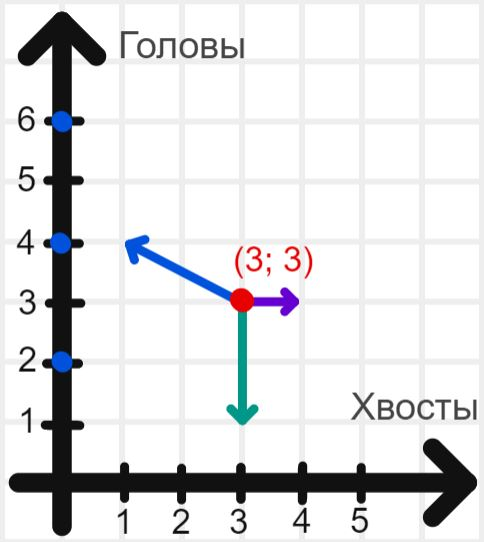
\includegraphics[width=\linewidth]{sol28}
        \end{figure}
    \end{minipage}
\end{minipage}
Можно отметить, что Змея можно победить за 9 ударов: если по разу выполнить действия 2-4, то количества хвостов и голов уменьшаются на 1.\\ После повторения этих трёх действий 3 раза Иван-Царевич побеждает.\smallskip\\
Быстрее победить Змея нельзя, вот строгое доказательство:\\ Пусть умный Иван-Царевич не выполняет действие №1 ни разу, всего $a$ раз отрубает один хвост (действие №2), $b$ раз отрубает два хвоста (действие №4), и $c$ раз отрубает 2 головы (действие №3). Тогда получаются уравнения для количества голов: $3 + b - 2c = 0\,$ и для количества хвостов: $3 + a - 2b = 0$.\\ Отсюда $a = 2b - 3$ и $b = 2c - 3$, откуда $a = 2\cdot(2c - 3) - 3 = 4c  - 9$.\\
$a$ должно быть неотрицательно (0 и больше) $\Rightarrow$ $c \geqslant 3$. Если $c = 3$, то $a = 12 - 9 = 3$ и $b = 3$, то есть всего как раз 9 действий. Если же $c \geqslant 4$, то $a \geqslant 16 - 9 = 7$, и если $a \geqslant 7$, а $c \geqslant 4$, то это уже никак не меньше $7 + 4 = 11$ действий в сумме.\\ Следовательно, надо минимум 9 ударов.}
{Нужно хотя бы 9 ударов.}{Полезно ввести координатную плоскость или неизвестные.}
\end{problem}

\begin{problem}{Координатная плоскость.}{6.9.3}{6K}{*}
{\vspace{-8mm}\\\begin{minipage}{\linewidth}
    \begin{minipage}{0.59\linewidth}

    На рисунке справа изображена линия на координатной плоскости $x0y$ (с осью $x$, осью $y$, и $0$).
    \smallskip\\a) Какова координата по оси $y$ у точки $S$ на этой линии, если её координата по оси $x$ равна $-1$?
    \smallskip\\b) Какова координата по оси $y$ у точки $P$ на этой линии, если её координата по оси $x$ равна $3$?
    \smallskip\\c) Какова координата по оси $x$ у точки $U$ на этой линии, если её координата по оси $y$ равна $-4$?

    \end{minipage}
    \hspace{0.02\linewidth}
    \begin{minipage}{0.38\linewidth}
        \begin{figure}[H]
        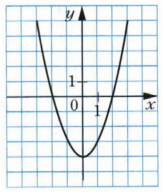
\includegraphics[width=\linewidth]{6K-3}
        \end{figure}
    \end{minipage}
\end{minipage}}
{НаписанноеРешение}
{ВерныйОтвет}{Подсказка}
\end{problem}

\begin{problem}{Графики.}{6.9.4}{6K}{*}
{Творческая задача: придумать, какая реальная ситуация может быть зарисована в виде графика, и схематично нарисовать этот график.}
{НаписанноеРешение}
{ВерныйОтвет}{Подсказка}
\end{problem}

\begin{problem}{Графики.}{6.9.4}{6K}{(лёгкая)}
{Творческая задача:\vspace{-11mm}\\
\begin{minipage}{\linewidth}
    \begin{minipage}{0.5\linewidth}
    ~\\~\\Чего не хватает графику, изображённому на рисунке справа?\medskip\\ Предложи вариант (или два), как можно исправить ситуацию.
    \end{minipage}
    \hspace{0.01\linewidth}
    \begin{minipage}{0.49\linewidth}
        \begin{figure}[H]
        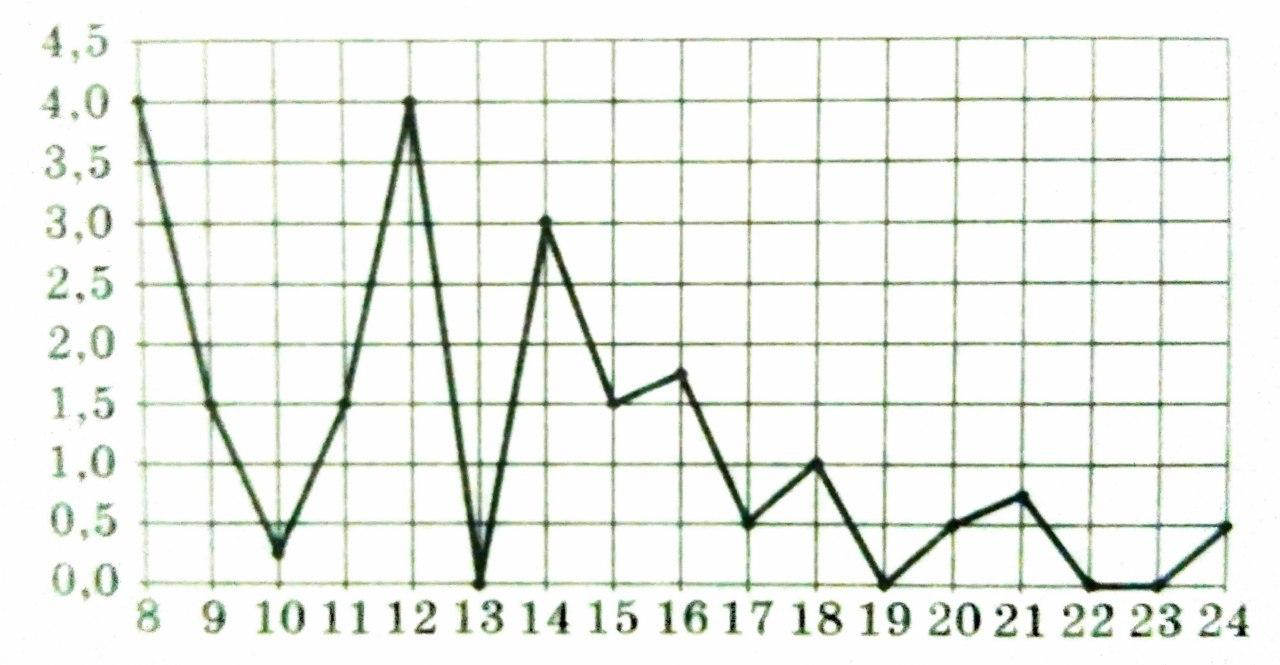
\includegraphics[width=\linewidth]{6K-36}
        \end{figure}
    \end{minipage}
\end{minipage}}
{НаписанноеРешение}
{ВерныйОтвет}{Подсказка}
\end{problem}

\begin{problem}{Графики.}{6.9.4}{6K}{*}
{Творческая задача: нарисовать график дневной температуры в Москве за последние две недели: по оси $x$ отложить дни, а по оси $y$~--- температуру (данные можно взять, например, на сайте \textcolor{CornflowerBlue}{\href{https://www.gismeteo.ru/diary/4368/}{\textbf{GISMETEO}}}).}
{Пример выполненного задания (температура за осень 2020 года):\\
    \begin{minipage}{\linewidth}
        \begin{figure}[H]
        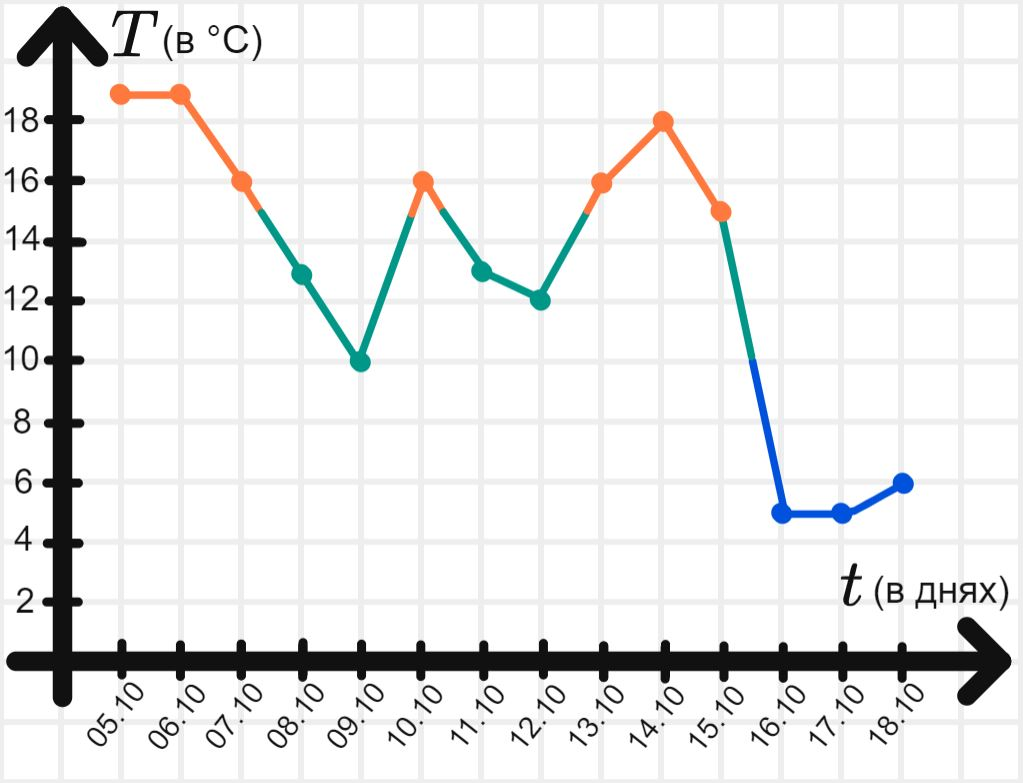
\includegraphics[width=\linewidth]{sol19}
        \end{figure}
    \end{minipage}
(Здесь оранжевым отмечена температура от 15 до 20$^\circ$C, зелёным~--- от 10 до 15$^\circ$C, тёмно-синим~--- от 5 до 10$^\circ$C.) Видно, что 16-ого октября существенно похолодало.}
{Смотри график выше.}{Изобразить нужно только дневную температуру.}
\end{problem}

\begin{problem}{Графики.}{6.9.4}{6K}{(лёгкая)}
{\vspace{-8mm}\\\begin{minipage}{\linewidth}
    \begin{minipage}{0.5\linewidth}
    \vspace*{10mm}
    Карантин закончился, и автомобилист едет с дачи в Москву (см. график).
    \smallskip\\Какое расстояние от дачи до Москвы?\\ Сколько времени автомобиль затратил на дорогу? Какова его средняя скорость?\smallskip\\

    \end{minipage}
    \hspace{0.01\linewidth}
    \begin{minipage}{0.49\linewidth}
        \begin{figure}[H]
        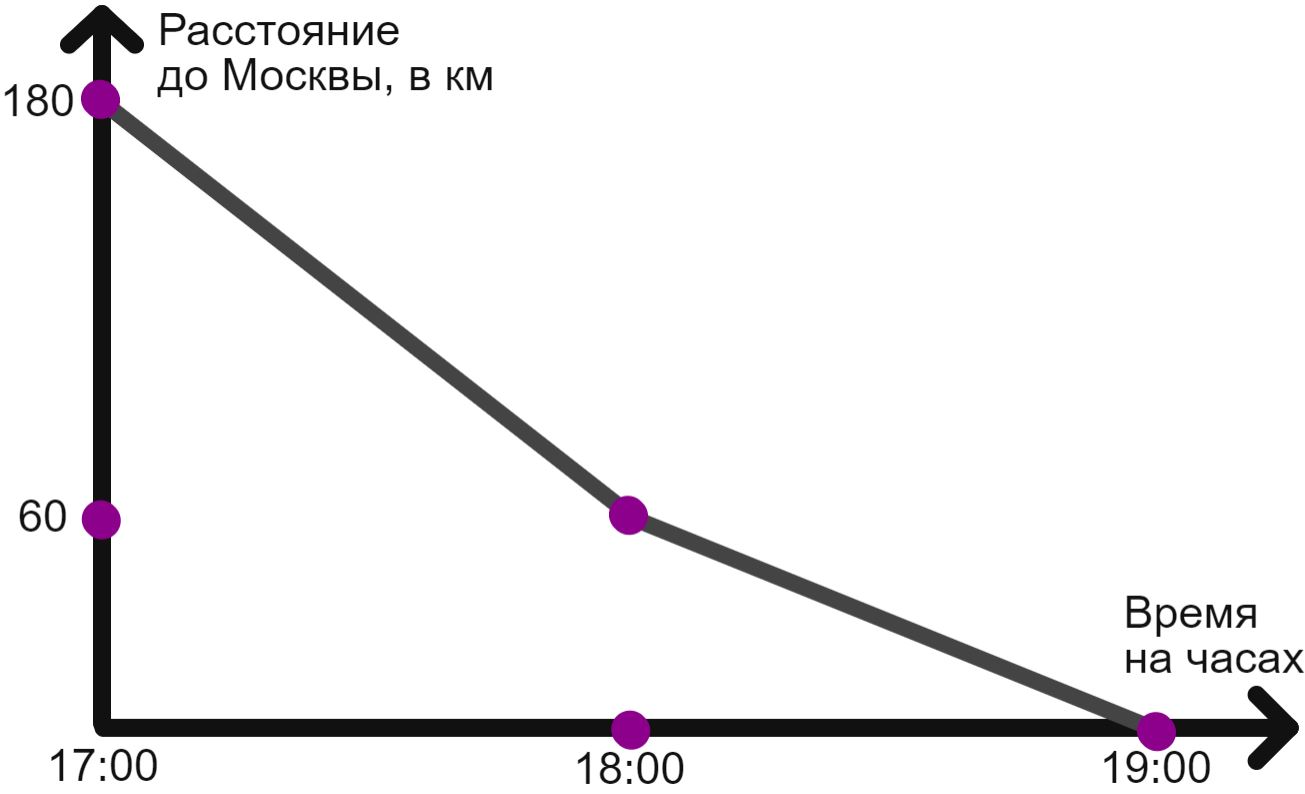
\includegraphics[width=\linewidth]{6K-9}
        \end{figure}
    \end{minipage}
\end{minipage}}
{Как мы можем видеть из графика, в самом начале его пути, когда автомобилист только выехал с дачи, до Москвы было 180 км~--- это и есть расстояние до Москвы. До Москвы он ехал 2 часа (с 17:00 до 19:00).\\ Средняя скорость равна $v = \frac{s}{t} = \frac{180}{2} = 90$ км/ч.}
{Расстояние от дачи до Москвы составляет 180 км, которые автомобилист проехал со средней скоростью $90$ км/ч за два часа.}{Средняя скорость равна $v_{\text{ср}} = \frac{s_{\text{общее}}}{t_{\text{пройденное}}}$.}
\end{problem}

\begin{problem}{Графики.}{6.9.4}{6K}{(лёгкая)}
{\vspace{-9mm}\\\begin{minipage}{\linewidth}
    \begin{minipage}{0.52\linewidth}
    \vspace*{10mm}
    Мотоциклист выехал из дома и через некоторое время вернулся назад. По дороге он два раза останавливался для отдыха.\smallskip\\ На рисунке справа изображён график изменения расстояния от дома в зависимости от времени (график движения мотоциклиста).
    \end{minipage}
    \hspace{0.02\linewidth}
    \begin{minipage}{0.45\linewidth}
        \begin{figure}[H]
        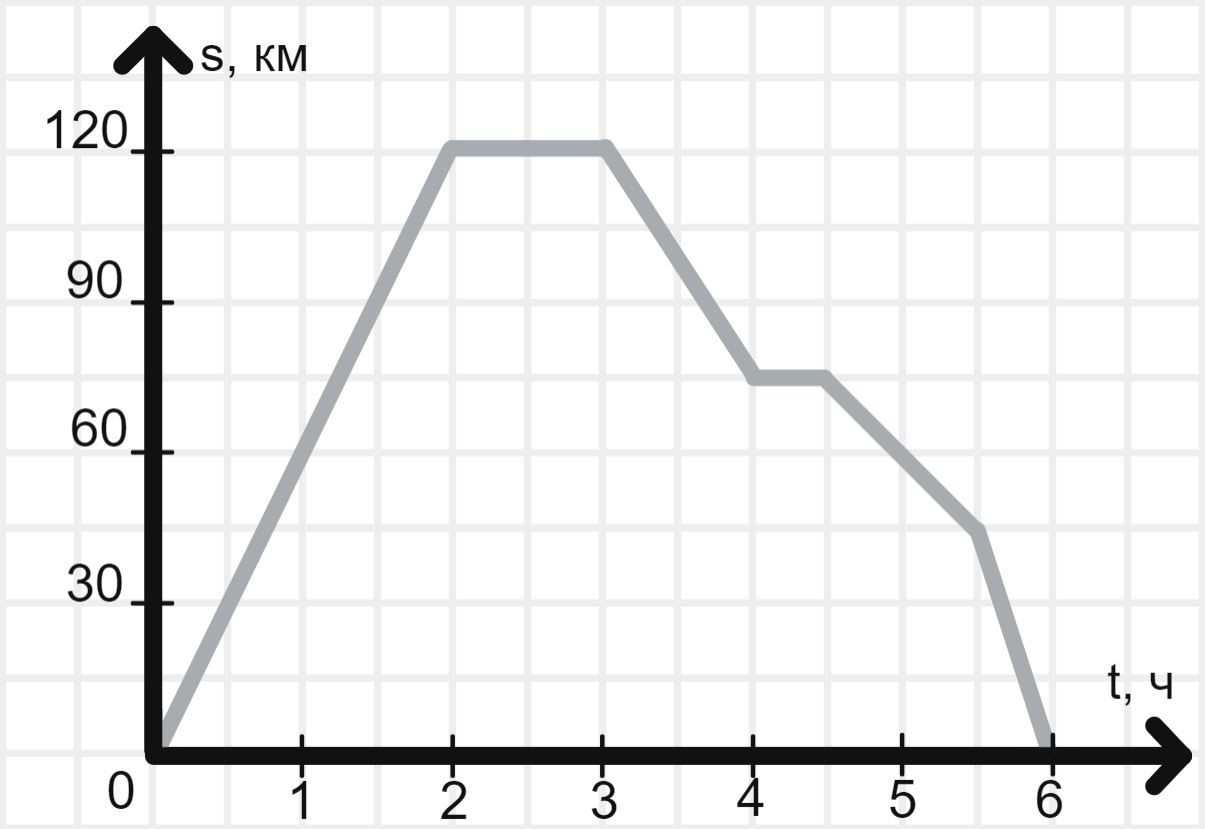
\includegraphics[width=\linewidth]{6K-4}
        \end{figure}
    \end{minipage}
\end{minipage}
\vspace{-5mm}\\Вопросы:\\
a) Какое расстояние проехал мотоциклист за первый час движения?\\
b) На каком расстоянии от дома мотоциклист останавливался отдыхать?\\
c) Сколько длился первый отдых? Второй отдых?\\
d) На каком расстоянии от дома был мотоциклист через $5$ часов после выезда?\\
e) С какой скоростью двигался мотоциклист последние полчаса?}
{НаписанноеРешение}
{ВерныйОтвет}{Подсказка}
\end{problem}

\begin{problem}{Графики.}{6.9.4}{6K}{(лёгкая)}
{\vspace{-8mm}\\\begin{minipage}{\linewidth}
    \begin{minipage}{0.47\linewidth}
    ~\vspace{6mm}\\
    На рисунке справа отображён график изменения температуры за пятницу, субботу и воскресенье июля 2018 года.\smallskip\\ В какой день выходных было теплее всего? Чему была равна температура?\smallskip\\ Какой была самая низкая температура за эти дни?

    \end{minipage}
    \hspace{0.02\linewidth}
    \begin{minipage}{0.5\linewidth}
        \begin{figure}[H]
        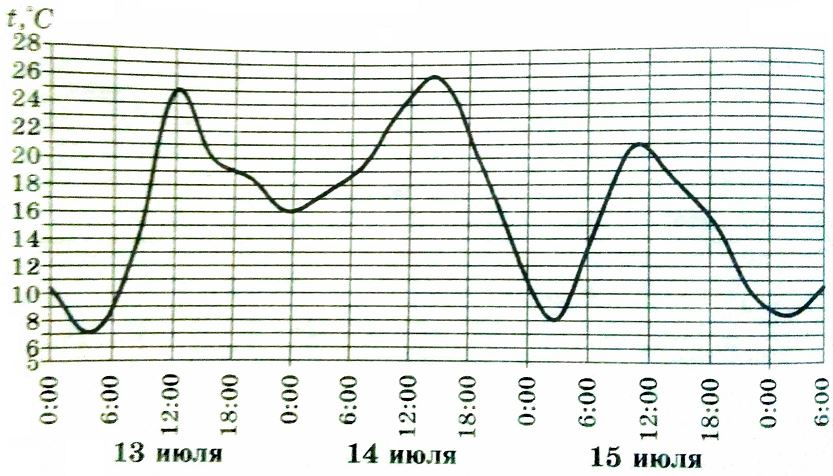
\includegraphics[width=\linewidth]{6K-37}
        \end{figure}
    \end{minipage}
\end{minipage}}
{НаписанноеРешение}
{ВерныйОтвет}{Подсказка}
\end{problem}

\begin{problem}{Графики.}{6.9.4}{6K}{(лёгкая)}
{На рисунке ниже изображен график изменения температуры в Квебеке (город в Канаде) в течение суток. \vspace{-4mm}\\\begin{minipage}{\linewidth}
    \begin{figure}[H]
    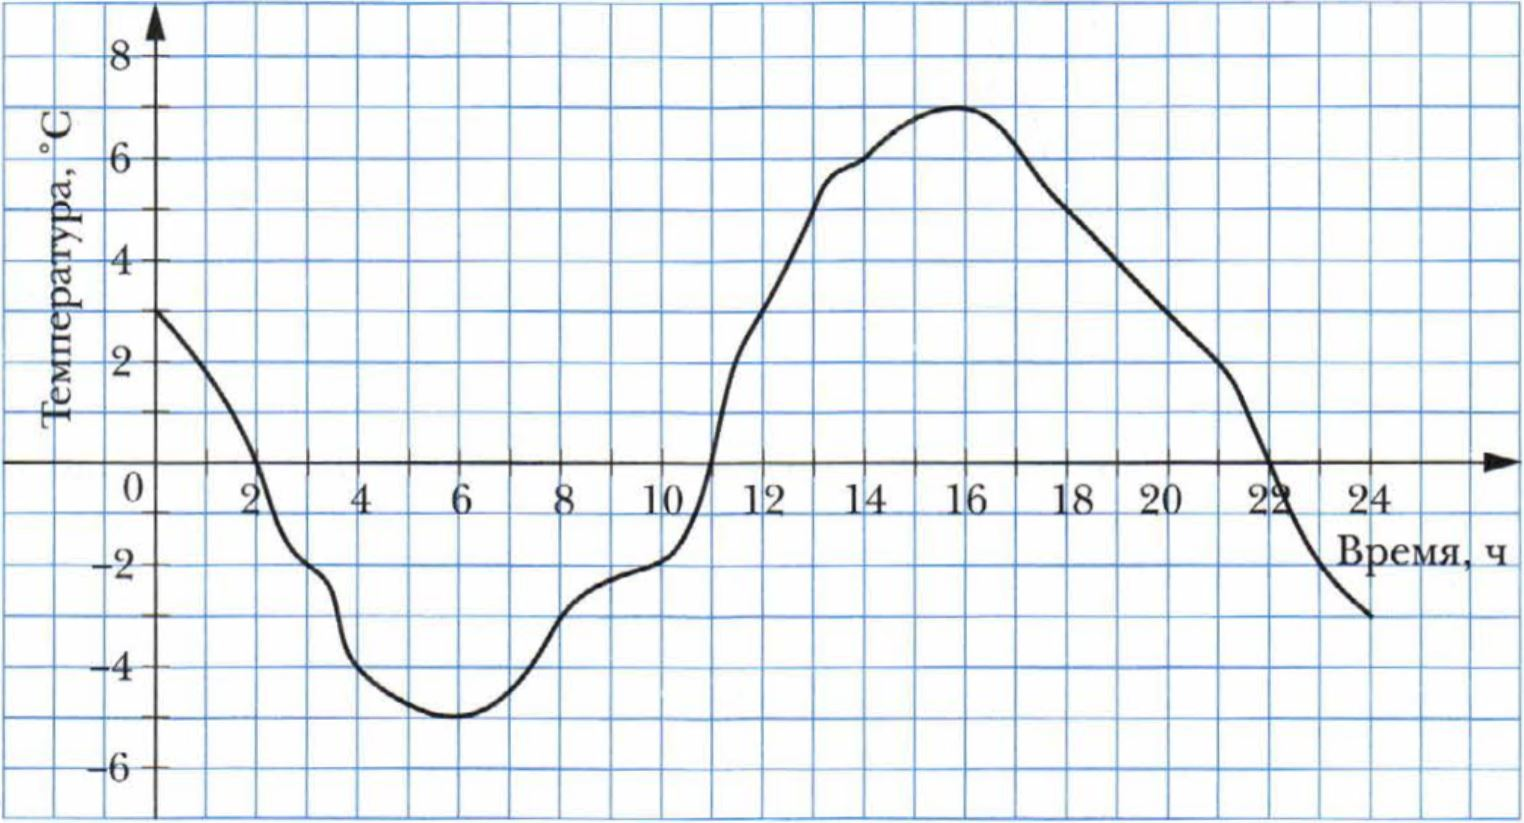
\includegraphics[width=\linewidth]{6K-6}
    \end{figure}
\end{minipage}
\vspace{-1mm}\\Пользуясь графиком, определить:
\\a) какой была температура воздуха в $4$ ч; в $6$ ч; в $10$ ч; в $13$ ч; в $18$ ч; в $22$ ч;
\\b) в котором часу температура воздуха была $3$ $C^{\circ}$; $-2$ $C^{\circ}$;
\\c) в котором часу температура воздуха была нулевой;
\\d) какой была самая низкая температура и в котором часу;
\\e) какой была самая высокая температура и в котором часу;
\\f) когда температура воздуха в Квебеке была ниже $0$ $C^{\circ}$; выше $0$ $C^{\circ}$;
\\g) в какие промежутки времени температура воздуха повышалась; понижалась.

}
{НаписанноеРешение}
{ВерныйОтвет}{Подсказка}
\end{problem}

\begin{problem}{Графики.}{6.9.4}{6K}{(лёгкая)}
{Велосипедист выехал из дома на прогулку. Сначала он ехал $2$ ч со скоростью $12$ км/ч, а потом отдохнул час и вернулся домой со скоростью $8$ км/ч.\\ Построить график движения велосипедиста.}
{НаписанноеРешение}
{ВерныйОтвет}{Подсказка}
\end{problem}

\begin{problem}{Графики.}{6.9.4}{6K}{(лёгкая)}
{На рисунке ниже в виде графика изображена зависимость пройденного туристами расстояния от времени.\vspace{-9mm}\\\begin{minipage}{\linewidth}
    \begin{minipage}{0.5\linewidth}
    ~\vspace*{8mm}\\
    Нужно найти: скорости туристов в разное время дня; общее время движения;\\ время, потраченное на остановки;\\ сколько времени было на часах, когда туристы сделали большой привал, собрали ведро грибов и сварили из них суп.
    \end{minipage}
    \hspace{0.05\linewidth}
    \begin{minipage}{0.44\linewidth}
        \begin{figure}[H]
        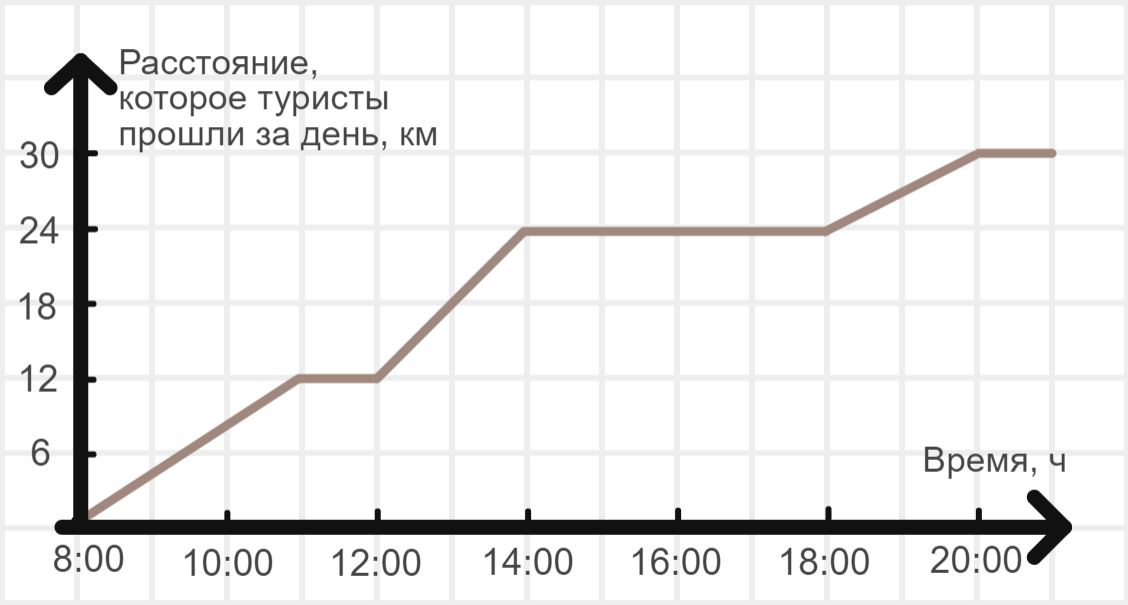
\includegraphics[width=\linewidth]{6K-7}
        \end{figure}
    \end{minipage}
\end{minipage}
~\vspace{-1mm}\\Когда туристы шли быстрее, утром или вечером?\\ Найти среднюю скорость движения туристов.}
{НаписанноеРешение}
{ВерныйОтвет}{Подсказка}
\end{problem}

\begin{problem}{Графики.}{6.9.4}{6K}{(лёгкая)}
{\vspace{-14mm}\\\begin{minipage}{\linewidth}
    \begin{minipage}{0.51\linewidth}
    ~\vspace{7mm}\\
    Некто едет по дороге в пробке, а затем выезжает из этой пробки и ещё три часа едет по свободной дороге (график его скорости изображён на рисунке справа).\smallskip\\ Сколько времени этот автомобилист стоял в пробке? Какое расстояние он проехал за всё время?
    \end{minipage}
    \hspace{0.04\linewidth}
    \begin{minipage}{0.44\linewidth}
        \begin{figure}[H]
        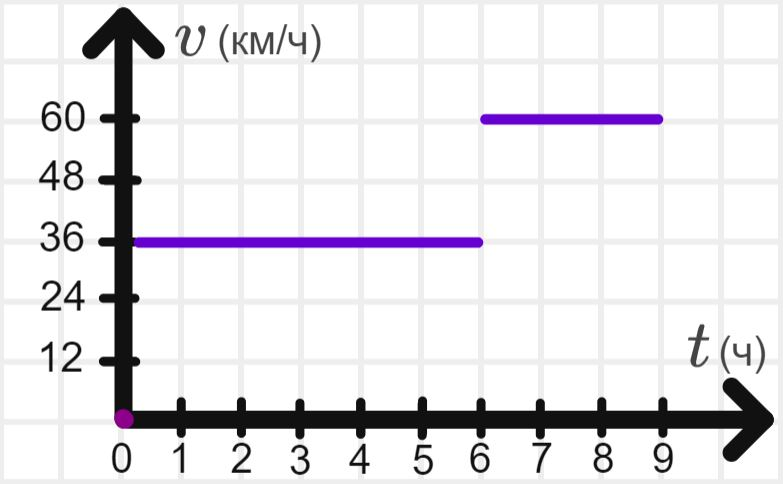
\includegraphics[width=\linewidth]{6K-8}
        \end{figure}
    \end{minipage}
\end{minipage}}
{Как мы можем видеть из графика, автомобилист ехал с одной и той же скоростью 36 км/ч 6 часов подряд~--- всё это время он стоял в пробке.\\
За всё время автомобилист проехал $s = 6\cdot36 + 3\cdot 60 = 216 + 180 = 396$ км.}
{Автомобилист проехал 396 км.}{$s = s_1 + s_2$.}
\end{problem}

\begin{problem}{Графики.}{6.9.4}{6K}{(лёгкая)}
{Туристы совершили поход на велосипедах за четыре дня.\\ В первый день они проехали $1/3$ всего пути без $2$ км. Во второй день~--- половину оставшегося пути без трёх километров. В третий день был сделан привал.\\ В четвёртый они проехали $8/9$ оставшегося пути и ещё $6$ км. \\Сколько всего километров проехали туристы за $4$ дня?\\ Нарисовать график их движения.}
{НаписанноеРешение}
{ВерныйОтвет}{Подсказка}
\end{problem}

\begin{problem}{Графики.}{6.9.4}{6K}{*}
{Белка за $20$ минут приносит орех в дупло. Далеко ли от гнезда до орешника, если налегке белка бежит со скоростью $5$ км/ч, а с орехом~--- со скоростью $3$ км/ч? Нарисовать график движения белки за час (белка стартует от дупла).}
{На то, чтобы сбегать от дупла до орешника и обратно, белка тратит 20 минут, или $\frac13$ часа. Пусть расстояние до орешника равно $s$. Тогда $\,\frac13 = \frac{s}{5} + \frac{s}{3}$.\\
Следовательно, $\frac13 = s\cdot\left(\frac15 + \frac13\right) \;\Rightarrow\; \frac13 = \frac{8}{15}\cdot s \;\Rightarrow\; s = \frac13 : \frac{8}{15} = \frac{1 \cdot 15}{3 \cdot 8} = \frac58 = 0{,}625$ км.\smallskip\\
Найдём, сколько времени белка бежит в одну сторону, а сколько в другую:\\ $\frac{s}{5} = \frac{1}{8}$ часа $= \frac{60}{8} = 7{,}5$ минут. $\;\frac{s}{3} = \frac{5}{24}$ часа $ = \frac{5 \cdot 60}{24} = \frac{25}{2} = 12{,}5$ минут.\\
Очевидно, что за час белка повторит это ровно три раза (в часе $60 = 20 \cdot 3$ минут).\smallskip\\
Отложим на графике по горизонтальной оси вправо время (в минутах), а по вертикальной оси~--- расстояние от белки до дупла (в метрах).\\
Полученный график изображён на рисунке ниже:\vspace{-2mm}\\
\begin{minipage}{\linewidth}
        \begin{figure}[H]
        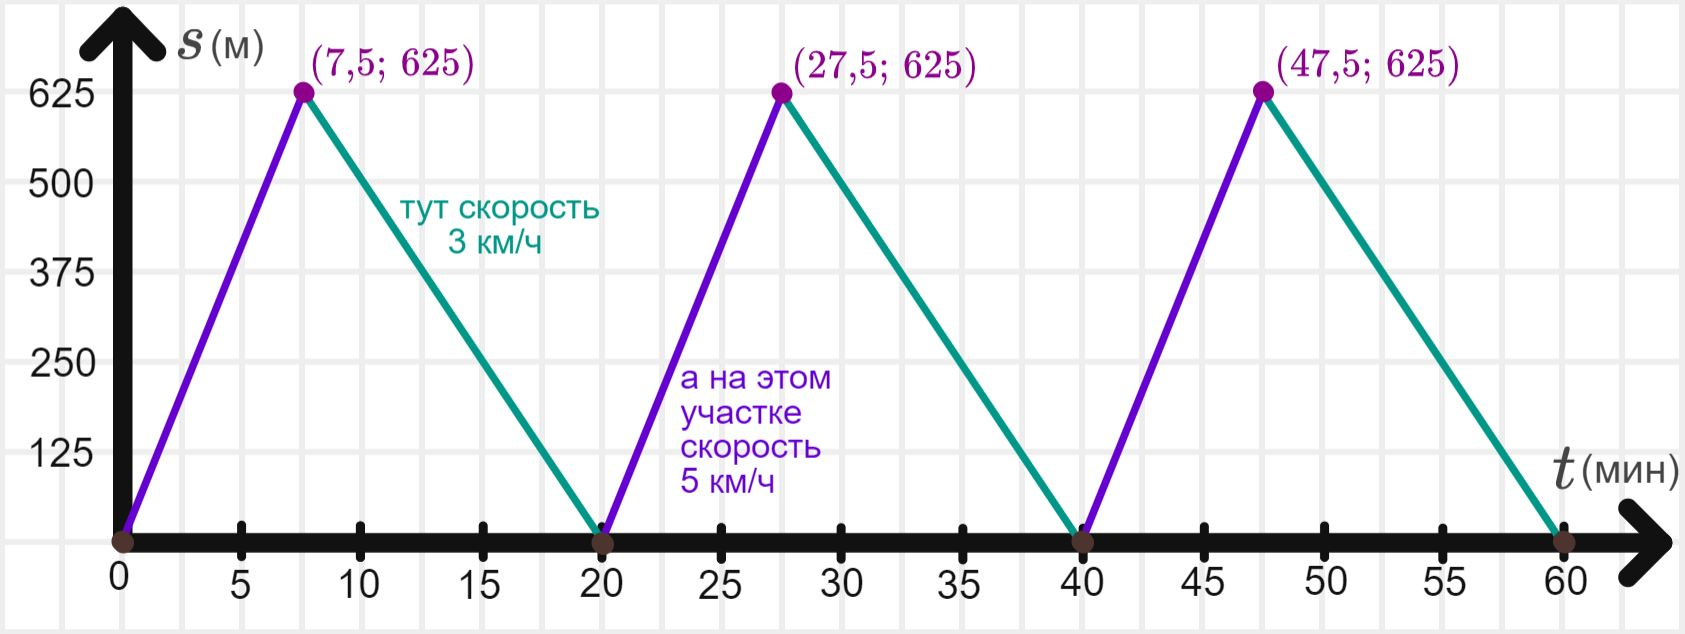
\includegraphics[width=\linewidth]{sol31}
        \end{figure}
    \end{minipage}}
{Расстояние от дупла до орешника составляет 625 метров.}{Белка вначале бежит от дупла до орешника, а потом сразу же\\ хватает очередной орех и бежит с ним обратно к дуплу.}
\end{problem}

\begin{problem}{Графики.}{6.9.4}{9I}{*}
{Улитка за день заползает вверх по дереву на 4 м, а за ночь сползает на 3 м.\\ Высота дерева 10 м, улитка начинает ползти с самого низа дерева.\\ Через сколько дней улитка впервые окажется на вершине?\\ Сколько раз за это время улитка окажется на высоте $5$ м над землёй?\\ Нарисовать график движения улитки.}
{\vspace{-12mm}\\\begin{minipage}{\linewidth}
    \begin{minipage}{0.51\linewidth}
    ~\vspace{7mm}\\
    Нарисуем график движения улитки, отложив по вертикали высоту дерева (что довольно логично), а по горизонтали~--- прошедшее время в днях.
    \end{minipage}
    \hspace{0.04\linewidth}
    \begin{minipage}{0.44\linewidth}
        \begin{figure}[H]
        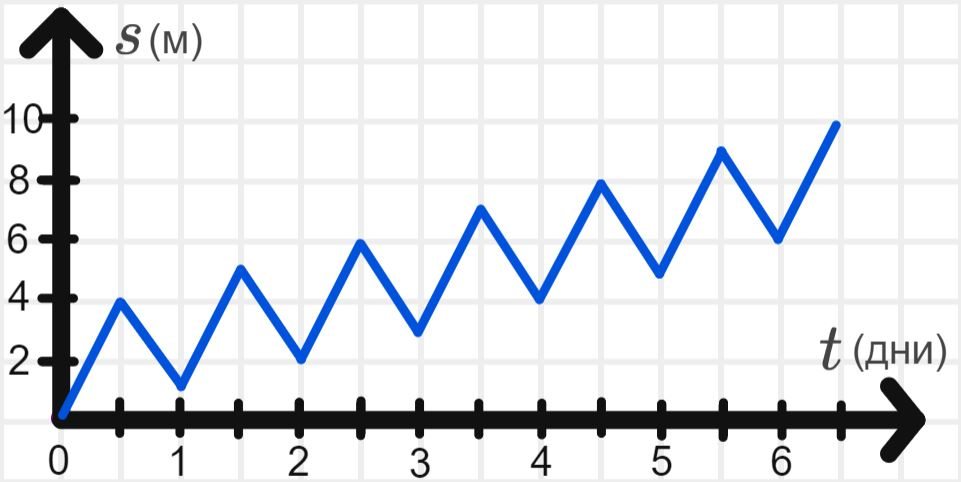
\includegraphics[width=\linewidth]{sol16}
        \end{figure}
    \end{minipage}
\end{minipage}
Получаем график, похожий на пилу, изображённый сверху. Из графика понятно, что за шесть полных дней улитка заползёт на 6 метров ($6\cdot(4-3)$), а на следующий день поднимется ещё на 4 метра и окажется на вершине. Таким образом, на вершине улитка окажется на седьмой день.\\ На высоте 5 метров улитка окажется 7 раз (достаточно посмотреть, сколько раз наш график имеет $s = 5$, то есть пересекает горизонтальную прямую)}
{Улитка окажется на вершине дерева на седьмой день.}{Улитка окажется на вершине раньше десятого дня.}
\end{problem}

\begin{problem}{Графики.}{6.9.4}{9I}{*}
{Две группы туристов (А и B) пошли в поход. В четвёртый день они по плану проходят мимо красивых водопадов, и группа А хочет потратить больше времени на то, чтобы их осмотреть, а группа B решает вообще не останавливаться.\vspace{-3mm}\\\begin{minipage}{\linewidth}
    \begin{minipage}{0.5\linewidth}
    Из-за этого группы разделяются и в этот день идут отдельно друг от друга.\smallskip\\ Всего за этот день им надо пройти до следующего места ночевки 18 км, график движения показан на рисунке справа.\smallskip\\ Группа А, для того чтобы успеть посмотреть водопады, выходит из лагеря на час раньше группы В.
    
    \end{minipage}
    \hspace{0.02\linewidth}
    \begin{minipage}{0.48\linewidth}
        \begin{figure}[H]
        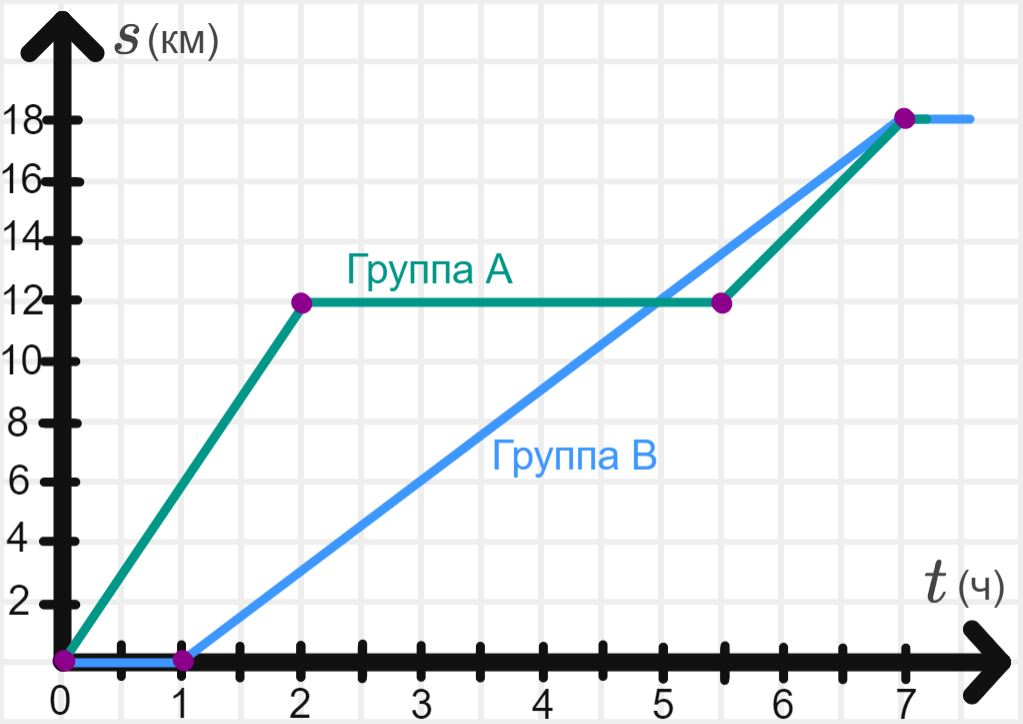
\includegraphics[width=\linewidth]{6K-47}
        \end{figure}
    \end{minipage}
\end{minipage}

\vspace{-4mm}
\textbf{Вопросы}:\\
\textbf{1)} Какова скорость группы А в первый час движения?\\
\textbf{2)} Сколько времени она потратила на осмотр водопадов?\\
\textbf{3)} Какова средняя скорость движения группы А?\\
\textbf{4)} На каком расстоянии от лагеря находятся водопады?\\
\textbf{5)} Сколько времени потратила группа В на то, чтобы дойти до них от лагеря?\\
\textbf{6)} Через какое время после того как группа В пройдёт мимо водопадов группа А продолжит движение? Какова средняя скорость движения группы В?\\
\textbf{7)} На каком максимальном расстоянии друг от друга будут находиться группы в течение этого дня? (подразумевается, что обе группы идут по одной и той же абсолютно прямой дороге, а водопады находятся рядом с ней)\\
\textbf{8)} Кто раньше окажется у следующего места ночёвки~--- группа А или группа В?}
{\textbf{1)} Из графика видно, что за первый час группа А отошла от лагеря на 6 километров. Следовательно, её скорость~--- 6 км/ч.\\
\textbf{2)} Во время осмотра водопадов группа находится на одном и том же расстоянии от лагеря (у водопадов). Как мы можем видеть на графике, группа А оказалась у водопадов через 2 часа после начала движения, а ушла от них через $5{,}5$ часов. Значит, группа А осматривала водопады $3{,}5$ часа.\\
\textbf{3)} За день группа А прошла 18 километров, потратив на это 7 часов.\\ Поэтому её средняя скорость равна $\frac{18}{7}$ км/ч.\\
\textbf{4)} Водопады находятся на расстоянии 12 километров от лагеря.\\
\textbf{5)} Группа В вышла на час позже группы А. То есть, она двигалась к водопадам с первого по пятый час, и всего затратила на это 4 часа.\\
\textbf{6)} Из графика видно, что обе группы находятся у водопадов через 5 часов после выхода группы А из лагеря. Поэтому группа А продолжит движение через полчаса. Группа В проходит 18 километров за 6 часов (первый час она просто сидит в лагере). Поэтому средняя скорость группы В равна $\frac{18}{6} = 3$ км/ч.\\
\textbf{7)} На графике расстояние до лагеря отложено по вертикали, поэтому разница по высоте между зелёной и синей ломаной и есть расстояние между группами.\\ Интуитивно понятно, что наибольшим это расстояние будет через 2 часа после начала движения группы А. К этому моменту группа А прошла 12 км (см. пункт 4), а группа В прошла 3 км (скорость движения группы В постоянна и равна 3 км/ч, см. пункт 6). Поэтому наибольшее расстояние между группами равно 9 км.\\
\textbf{8)} Ровно через 7 часов после начала движения обе группы останавливаются.\\ Таким образом, до следующего места ночёвки они дошли одновременно.}
{Смотри решение выше.\\
\textit{Комментарий:} если считать, что средняя скорость должна рассчитываться только за время движения, то в пункте 3 получится другой ответ, так как тогда расстояние в 18 км было пройдено за $7 - 3{,}5 = 3{,}5$ часа, и средняя скорость движения группы А будет равна $\frac{18}{3{,}5} = \frac{36}{7}$ км/ч.}{Следует внимательно изучить график.}
\end{problem}

\begin{problem}{Графики.}{6.9.4}{6K}{*}
{Найти точки $(x; y)$, которые являются решениями уравнения $y = x^{2}$, и попробовать их нарисовать на координатной плоскости (но стоит иметь в виду, что $y$ здесь всегда положителен, а вот $x$ может быть и положительным, и отрицательным).}
{НаписанноеРешение}
{ВерныйОтвет}{Подсказка}
\end{problem}

\end{document}